	\documentclass[twoside]{article}
\usepackage{../../estilo-ejercicios}
\renewcommand{\baselinestretch}{1,4}
%--------------------------------------------------------
\begin{document}

\title{Ejercicios de Algebraic Geometry, Capítulo 2, Sección 3}
\author{Javier Aguilar Martín}
\maketitle


%\begin{ejercicio}{1.1}

%\end{ejercicio}
%\begin{solucion}
%
%\end{solucion}
%
%\newpage
%
%
%\begin{ejercicio}{1.2}
%
%\end{ejercicio}
%\begin{solucion}
%
%\end{solucion}
%
%\newpage
%DECIRLE QUE QUIERO HACER EL 2.16


%\begin{ejercicio}{3.1}
%Probar que un morfismo $f:X\to Y$ es localmente de tipo finito si y solo si para \emph{todo} abierto afín $V=\spec(B)$ de $Y$, $f^{-1}(V)$ puede ser cubierto por abiertos afines $U_j=\spec(A_j)$, donde cada $A_j$ es una $B$-álgebra finitamente generada. 
%\end{ejercicio}
%\begin{solucion}
%Una de las implicaciones es trivial, así que supongamos que $f:X\to Y$ es localmente de tipo finito. Sea $V=\spec(B)$ un abierto afín de $Y$ y consideremos $f^{-1}(V)$. Por ser $f$ localmente de tipo finito, podemos recubrir $Y$ con abiertos afines $V_i=\spec(B_i)$ de modo que $f^{-1}(V_i)$ está cubierto por abiertos afines $U_{ij}=\spec(A_{ij})$, donde cada $A_{ij}$ es na $B_i$-álgebra finitamente generada. %Esto nos da un recubrimiento de $f^{-1}(V)$ por abiertos de $X$, ya que $f^{-1}(V)=f^{-1}(V\cap \bigcup V_i)=\bigcup(f^{-1}(V)\cap f^{-1}(V_i))$, pero estos abiertos no tienen por qué ser afines. 
%
%Observemos que para $\p\in B_i$, $f^{-1}(\spec((B_i)_\p))$ está cubierto por los $f^{-1}(\spec((A_{ij})_{\p^e})$, donde el ideal $\p^e$ es el extendido de $\p$ por la aplicación del álgebra $B_i\to A_{ij}$: si $f(x)\in\spec((B_i)_{\p})$, entonces $f(x)$ es un primo de $B_i$ que no contiene a $\p$, por lo que 

%\url{https://math.stackexchange.com/questions/384137/intersection-of-open-affines-can-be-covered-by-open-sets-distinguished-in-both}
%\url{https://math.arizona.edu/~cais/CourseNotes/AlgGeom04/Hartshorne_Solutions.pdf}
%\url{https://math.stackexchange.com/questions/2588088/prime-ideals-of-a-localization}
%
%
%NUEVA IDEA
%
%
%\url{http://mathbabysteps.blogspot.com/2016/12/affine-communication-lemma.html}
%\url{https://math.stackexchange.com/questions/803636/question-on-morphism-locally-of-finite-type}

%Una de las implicaciones es trivial, así que supongamos que $f:X\to Y$ es localmente de tipo finito. Sea $V=\spec(B)$ un abierto afín de $Y$. Del recubrimiento afín $\{V_i=\spec(B_i)\}_{i\in I}$ de $Y$ que nos da que $f$ sea localmente de tipo finito obtenemos un recubrimiento afín de $V$, pero $V\cap V_i$ no será en general afín, así que necesitamos el siguiente lema:
%
%\begin{lemma}
%Sean $U=\spec(A)$ y $V=\spec(B)$ subesquemas afines abiertos de un esquema $X$. Entonces $\spec(A)\cap\spec(B)$ puede ser recubierto por abiertos $W_i$ que son subesquemas abiertos básicos tanto de $\spec(A)$ como de $\spec(B)$.
%\end{lemma}
%\begin{proof}
%Hacemos primero la siguiente observación: dado un abierto $U$ y $g\in\OO_X(U)$ y $V\subseteq U$, denotamos $U_g=\{x\in U\mid g_x\notin \mm_x\}$ donde $\mm_x$ es el ideal maximal de $\OO_x$, entonces $U_g\cap V=V_{g|_V}$. 
%
%Sea $p\in\spec(A)\cap\spec(B)$. Afirmamos que existe un subesquema abierto básico tanto de $\spec(A)$ como de $\spec(B)$ conteniendo a $x$. Sea $\spec(A)\supseteq\spec(A_f)\ni p$ y sea $\spec(A_f)\supseteq\spec(B_g)\ni p$ tal como se observa en la figura.
%\begin{figure}[h!]
%\centering
%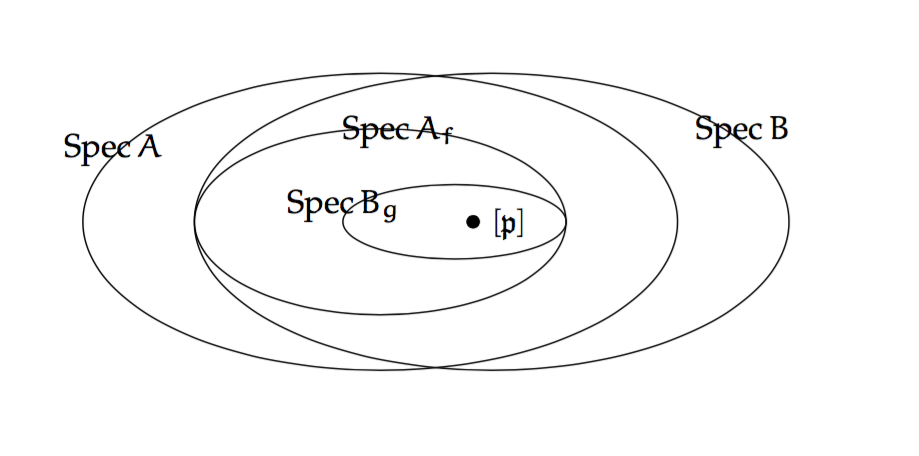
\includegraphics[scale=0.22]{3-1}
%\end{figure}
%
% Estas inclusiones y el hecho de que $\spec(A_f)$ es básico en $\spec(A)$ y $\spec(B_g)$ es básico en $\spec(B)$ nos lo da el ejercicio 2.1. Vamos a probar que $\spec(B_g)$ también es básico en $\spec(A)$. Tenemos que $g\in\Gamma(\spec(B),\OO_X)$ se restringe a $g'\in\Gamma(\spec(A_f),\OO_X)=A_f$. Por la observación del principio de la demostración tenemos que $\spec(B_g)=\spec(A_f)_{g'}$. Si $g'=g''/f^n$ con $g''\in A$, tal como se hizo en el apartado (a) del ejercicio 2.16 se prueba que además $\spec(A_f)_{g'}=\{x\in\spec(A)\mid (f^ng'')_x=g'_x\notin \mm_x\}=D(g')$, con lo que hemos probado el resultado. 
%
%
%
%\end{proof}
%Ahora podemos cubrir $V$ con subesquemas afines que son básicos tanto en $V$ como en $V_i$, y tomando preimágenes recubrimos $f^{-1}(V)$ (aunque cada preimagen no tiene por qué ser afín). Sea $V'$ unos de esos subesquemas afines, digamos $D(g)=V'= D(g_i)$ con $g\in B$ y $g_i\in B_i$. Podemos cubrir $f^{-1}(V')$ por subesquemas affines abiertos que son abiertos básicos para unos ciertos abiertos afines $U_{ij}=\spec(A_{ij})$ de $X$ (los que nos da que $f$ sea localmente de tipo finito). Sea $U'$ uno de esos abiertos básicos, digamos $U'=D(f_{ij})$ para $f_{ij}\in A_{ij}$. 
%
%Ahora, $f|_{U_{ij}}:U_{ij}\to V_i$ está inducida por un homomorfimos de anillos $\varphi_{ij}:B_i\to A_{ij}$ por la proposición 2.3(c), por lo que $A_{ij}$ es una $B_i$-álgebra. Como $U'\subseteq f^{-1}(V\cap V_i)$, sabemos que $f|_{U'}:U'\to V_i$ está inducida por la localización de $\varphi_{ij}$, pero también por un cierto homomorfismo $\varphi:B\to (A_{ij})_{f_{ij}}$. Probaremos que esto convierte a $A=(A_{ij})_{f_{ij}}$ en una $B$-álgebra finitamente generada.
%
%Usamos que $U'\subseteq f^{-1}(V')$ para obtener dos homomorfismos de anillos inducidos por $f$, $\psi:B_g\to A$ y $\psi_{ij}:(B_i)_{g_i}\to A$. De la construicción de $V'$ y $U'$ se sigue que $\psi$ es la localización de $\varphi$ y $\psi_{ij}$ la localización de $\varphi_{ij}$ compuesta con la localización $A_{ij}\to A$. Además, si $\sigma:B_g\to (B_i)_{g_i}$ es el isomorfismo inducido por el isomorfismo de sus espectros, $\psi=\psi_{ij}\circ\sigma$ por la conmutatividad de los morfismos de esquemas
%\[
%\begin{tikzcd}
%D(g)& D(f_{ij})\arrow[l, "f"']\arrow[dl, "f"]\\
%D(g_i)\arrow[u, equals] & 
%\end{tikzcd}
%\]
%
%Finalmente, por hipótesis tenemos que $A_{ij}$ es una $B_i$-álgebras finitamente generadas, con lo que también lo es $A=(A_{ij})_{f_{ij}}$. Pero entonces también es un una $(B_i)_{g_i}$-álgebra finitamente generada, lo cual es equivalente a ser una $B_g$-álgebra finitamente generada, y entonces es una $B$-álgebra finitamente generada, como queríamos probar.
%\end{solucion}
%
%\newpage




%
%
%
%
%\end{solucion}
%

%
%\begin{ejercicio}{2.16}
%
%\end{ejercicio}
%\begin{solucion}
%Un morfismo de esquemas $f:X\to Y$ es \emph{quasi-compacto} si existe un recubrimiento de $Y$ por abiertos afines $V_i$ tales que $f^{-1}(V_i)$ es quasi-compacto para cada $i$. Porbar que $f$ es quasi-compacto si y solo si para \emph{todo} abierto afín $V\subseteq Y$, $f^{-1}(V)$ es quasi-compacto.
%\end{solucion}
%%
%\newpage
%%
%\begin{ejercicio}{Lema de Yoneda}
%$h_*:\CC\to \mathrm{Fun}(\CC^{op}, \mathrm{Set})$ es plenamente fiel, es decir, para todo $X,X'\in Ob(\CC)$ la aplicación $\alpha\in\Hom_{\CC}(X,X')\mapsto h_{\alpha}\in \mathrm{Nat}(h_X,h_{X'})$ es un isomorfismo. 
%\end{ejercicio}
%\begin{solucion}
%%https://math.stackexchange.com/questions/94007/proof-of-yoneda-lemma
%Supongamos que existen $\alpha,\alpha'\in\Hom(X,X')$ tales que $h_\alpha=h_{\alpha'}$. Tenemos entonces, un diagrama conmutativo
%\[
%\begin{tikzcd}
%h_X(X)\arrow[r, "h_\alpha=h_{\alpha'}"]\arrow[d, "h_X(Id)"'] & h_{X'}(X)\arrow[d, "h_{X'}(Id)"]\\
%h_X(X)\arrow[r, "h_\alpha=h_{\alpha'}"'] & h_{X'}(X)
%\end{tikzcd}
%\]
%Dada una flecha $f\in h_X(X)$, $$h_{X'}\circ h_{\alpha}(f)=\alpha\circ f\circ Id=\alpha\circ f$$
%$$h_{X'}\circ h_{\alpha'}(f)=\alpha'\circ f\circ Id=\alpha'\circ f$$
%En particular, para $f=Id:X\to X$, obtenemos $\alpha=\alpha'$, y con ello la inyectividad. 
%
%Sea ahora $\tau:h_X\to h_{X'}$ una transformación natural cualquiera, de modo que tenemos el diagrama conmutativo para todo $U,V\in Ob(\CC)$  y $f\in\Hom_{\CC^{op}}(U,V)$ 
%\[
%\begin{tikzcd}
%h_X(U)\arrow[r, "\tau(U)"] \arrow[d, "h_X(f)"']& h_{X'}(U)\arrow[d, "h_{X'}(f)"]\\
%h_X(V)\arrow[r, "\tau(V)"'] & h_{X'}(V)
%\end{tikzcd}
%\]
%donde $h_X(f)$ se debe interpretar como $h_X(f^{op})$. En particular, para $U=X$ tenemos por el diagrama que $\tau(U)\circ h_X(f)=h_{X'}(f)\circ\tau(X)$. Definimos $\alpha=\tau(X)(Id)\in h_{X'}(X)=\Hom(X,X')$. Sustituyendo $Id$ en el lado izquierdo de la ecuación de conmutatividad obtenemos
%\[
%\tau(U)\circ h_X(f)(Id)=\tau(U)( f^{op})
%\]
%y en el lado derecho
%\[
%h_{X'}(f)\circ\tau(X)(Id)=h_{X'}(f)(\alpha)=\alpha\circ f^{op}=h_\alpha(f^{op})
%\]
%Como esto se tiene para toda $f$, obtenemos que $h_\alpha=\tau(U)$, y como esta igualdad es para todo $U$, deducimos que $\tau=h_{\alpha}$, lo que nos da la sobreyectividad. 
%\end{solucion}
%
\newpage
%
\begin{ejercicio}{3.12}\emph{Subesquemas cerrados de $\proj(S)$}
\begin{enumerate}
\item[(a)]Sea $\varphi:S\to T$ un homomorfismo sobreyectivo de anillos graduados preservando grados. Probar que el abierto $U$ del ejercicio 2.14 es igual a $\proj(T)$, y que el morfismo $f:\proj(T)\to\proj(S)$ es una inmersión cerrada.
\item[(b)] Si $I\subseteq S$ es un ideal homogéneo, sea $T=S/I$ y sea $Y$ un subesquema cerrado de $X=\proj(S)$ definido como la imagen de la inmersión cerrada $\proj(S/I)\to X$. Probar que diferentes ideales homogéneos pueden dar lugar al mismo subesquema cerrado. Por ejemplo, sea $d_0$ un entero y sea $I'=\bigoplus_{d\geq d_0}I_d$. Probar que $I$ e $I'$ determinan el mismo subesquema cerrado.
\end{enumerate}
\end{ejercicio}
\begin{solucion}\
\begin{enumerate}[(a)]
\item Recordamos que $U=\{\p\in\proj(T)\mid \p\not\supseteq\varphi(S_+)\}$ y que por el ejercicio 2.14 $U$ es un subconjunto abierto de $\proj(T)$. Como $\varphi$ es sobreyectivo y gradudado, necesariamente se tiene $\varphi(S_+)=T_+$, por lo que por la definición de $\proj(T)$ se tiene la igualdad. Recordamos también que el morfismo $f:U\to\proj(S)$ está definido mediante la contracción $\p\in U\mapsto f(\p)=\varphi^{-1}(\p)$, que es continua de manera análoga al morfismo definido de esta forma para $\spec$. 

Por otro lado, como $S/\ker\varphi\cong T$ y los ideales primos homogéneos de $S/\ker\varphi$ se corresponden biunívocamente con los ideales primos homogéneos de $S$ que contienen a $\ker\varphi$, deducimos que $f:\proj(T)\to\proj(S)$ es un homeomorfismo sobre $V(\ker\varphi)$, y como $\ker\varphi$ es un ideal homogéneo al ser $\varphi$ graduado, $V(\ker\varphi)$ es un cerrado de $\proj(S)$. Falta ver que el homomorfismo $f^\sharp:\OO_{\proj(S)}\to f_*\OO_{\proj(T)}$ es sobreyectivo. 

Para ello es suficiente probarlo en las fibras, que por el ejercicio 1.8 es equivalente a probarlo para los homomorfismos $\OO_{\proj(S),\varphi^{-1}(\p)}\to\OO_{\proj(T),\p}$ usando que $f^{-1}(\OO_{\proj(S)})_{\p}=\OO_{\proj(S),f(\p)}$. Ahora bien, por la proposición 2.5 tenemos que esta aplicación es la aplicación $S_{(\varphi^{-1}(\p))}\to T_{(\p)}$ inducida por $\varphi$, por lo que es claramente sobreyectiva.


%Si nos restringimos a un abierto principal $D_+(g)$ para $g\in S$, tenemos por la proposición 2.5 que $\OO_{\proj(S)}(D_+(g))=S_{(g)}$ y $f_*\OO_{\proj(T)}(D_+(g))=\OO_{\proj(T)}(f^{-1}(D_+(g)))=T_{(\varphi(g))}$ ESTO ALOMEJOR LO DESARROLLO MÁS (por ser $\varphi$ sobreyectivo $\varphi(g)$ es un ideal). Esto nos da un homomorfismo natural $S_{(g)}\to T_{(\varphi(g))}$, que es claramente sobreyectivo por serlo $\varphi$. 

\item Consideremos la proyección natural $\varphi:S/I'\to S/I=\dfrac{S/I}{\oplus_{d\leq d_0}I_d}$ (usamos aquí la graduación inducida en el cociente). Es claro que $\varphi$ es un homomorfismo graduado, y denotamos por $\varphi_d$ a cada componente homogénea de $\varphi$. Entonces $\varphi_d$ es la identidad para $d>d_0$, así que usando el ejercicio 2.14 c), $f:\proj(S/I)\to\proj(S/I')$ es un isomorfismo. 

%Por la proposición 2.5 este homomorfismo es equivalente a $f^\sharp:S_{(\varphi^{-1}(p)}$ %Por la proposición 2.5, este homomorfismo des de la forma $f^\sharp:S_{(f)}\to T_{}
\end{enumerate}

\end{solucion}
%\newpage
%\begin{ejercicio}{3.17}\emph{Espacios de Zariski}. 
%
%
%\end{ejercicio}
%\begin{solucion}
%%
%\end{solucion}

\newpage

\begin{ejercicio}{3.22}\emph{Dimensión de las fibras de un morfismo.} Sea $f:X\to Y$ un morfismo dominante de esquemas íntegros de tipo finito sobre un cuerpo $k$. 
\begin{enumerate}[(a)]
\item Sea $Y'$ un subconjunto cerrado irreducible de $Y$, cuyo punto genérico $\eta'$ está contenido en $f(X)$. Sea $Z$ una componente irreducible de $f^{-1}(Y)$ tal que $\eta'\in f(Z)$. Probar que $\mathrm{codim}(Z,X)\leq \mathrm{codim}(Y',Y)$. 
\item Sea $e=\dim(X)-\dim(Y)$ la \emph{dimensión relativa} de $X$ sobre $Y$. Para cualquier punto $y\in f(X)$, probar que toda componente irreducible de la fibra $X_y$ tiene dimensión $\geq e$. [Pista: sea $Y'=\overline{\{y\}}$ y usar (a) y el ejercicio 3.20b]
\item Probar que existe un abierto denso $U\subseteq X$ tal que para cualquier $y\in f(U)$, $\dim(U_y)=e$. [Pista: primero reducir al caso en el que $X$ e $Y$ son afines, digamos $X=\spec(A)$ e $Y=\spec(B)$. Entonces $A$ es una $B$-álgebra finitamente generada. Tomar $t_1,\dots, t_e\in A$ que forman una base de transcendencia de $K(X)$ sobre $K(Y)$, y sea $X_1=\spec(B[t_1,\dots, t_e]$. Entonces $X_1$ es isomorfo al $e$-espacio afín sobre $Y$, y el morfismo $X\to X_1$ es generalmente finito. Ahora usar el ejercicio 3.7]
\item Volviendo al morfismo original $f:X\to Y$, para cualquier entero $h$, sea $E_h$ el conjunto de puntos $x\in X$ tales que, escribiendo $y=f(x)$, hay una componente irreducible $Z$ de la fibra $X_y$ conteniendo a $x$ y con $\dim(Z)\geq h$. Probar que
\begin{enumerate}
\item $E_e=X$ (usar (b)),
\item si $h>e$, entonces $E_h$ no es denso en $X$ (usar (c)),
\item $E_h$ es cerrado para todo $h$ (usar inducción en la dimensión de $X$).
\end{enumerate}
\item Probar el siguiente teorema de Chevalley---ver Cartan y Chevalley [1, exposé 8]. Para cada entero $h$, sea $C_h$ el conjunto de puntos $y\in Y$ tales que $\dim X_y=h$. Entonces los subconjuntos $C_h$ son constructibles y $C_e$ contiene un subconjunto abierto denso de $Y$.
\end{enumerate}

\end{ejercicio}
\begin{solucion}\
\begin{enumerate}[(a)]
\item Vamos a ver que una cadena de subconjuntos cerrados irreducibles distintos de $X$ empezando en $Z$ da lugar a una cadena de subconjuntos cerrados irreducibles distintos de $Y$ empezando en $Y'$. Supongamos que existe un cerrado irreducible $Z_1\subseteq X$ tal que $Z<Z_1$. Sea $Y_1=\overline{f(Z_1)}$, que es obviamente cerrado. Veamos que $Y_1$ es irreducible. Esto se debe a que por ser $Z_1$ irreducible, $f(Z_1)$ también lo es (imagen continua de un irreducible es irreducible), y la clausura de un irreducible es también irreducible. 

Por último veamos que $Y'<Y_1$. En primer lugar, $Y'=\overline{f(Z)}$: como $\eta'\in f(Z)$ sabemos que $Y'=\overline{\{\eta'\}}\subseteq\overline{f(Z)}$, mientras que la inclusión opuesta se obtiene de que $f(Z)\subseteq f(f^{-1}(Y'))\subseteq Y'$, y al ser $Y'$ cerrado la contención se preserva al tomar clausura. En segundo lugar, obsérvese que $Y'\subseteq Y_1$ ya que $Z<Z_1$ implica $f(Z)\subseteq f(Z_1)$. Para ver que la contención es estricta, el hecho de que $Z$ sea una componente irreducible de $f^{-1}(Y')$, significa que $Z$ es un subconjunto irreducible de $f^{-1}(Y')$ que además es maximal con respecto a la inclusión. Si tuviéramos $Y'=Y_1$, $Z<Z_1$ contradeciría la maximalidad de $Z$, ya que $Z_1$ estaría contenido en $f^{-1}(Y')$ y sería una componente irreducible estrictamente mayor que $Z$.

Por tanto la cadena $Z<Z_1$ induce una cadena $Y'<Y_1$. Podemos continuar este proceso inductivamente para cualquier cadena de subconjuntos cerrados irreducibles distintos de $X$ que comience en $Z$, dando lugar a una cadena análoga en $Y$ comenzando por $Y'$, por lo que se tiene la desigualdad deseada. 

\item Por el ejercico 3.10a, al ser la dimensión una propiedad topológica, basta demostrar el resultado para el espacio topológico $f^{-1}(y)$ con la topología inducida. Siguiendo la pista del ejercicio, dado $y\in f(X)$, denotamos $Y'=\overline{\{y\}}$. Sea $Z$ una componente irreducible de $f^{-1}(Y')$ tal que $y\in Z$ (en este caso $y$ es el punto genérico de $Y'$ por definición). Por el apartado (a) tenemos que $\codim(Z,X)\leq\codim(Y',Y)$. Por el ejercicio 3.20d tenemos que $\dim(Z)+\codim(Z,X)=\dim(X)$ y $\dim(Y')+\codim(Y',Y)=\dim(Y)$, luego combinando estas desigualdades junto con (a) obtenemos
\[
\dim(X)-\dim(Z)\leq\dim(Y)-\dim(Y')
\]
de donde $e=\dim(X)-\dim(Y)\leq \dim(Z)-\dim(Y')\leq\dim(Z)$. 

Sea ahora $W$ una componente irreducible de $f^{-1}(y)$. Sean $k$ la codimensión de $\overline{W}$ (clausura en $X$) en $X$ y sea $k'$ la codimensión de $Y'$ en $Y$. Ahora, $\overline{W}$ es una componente irreducible de $f^{-1}(Y')$ . Por (a) tenemos que $k\leq k'$. Aplicando el ejercicio 3.20b y la aditividad del grado de transcendencia en torres obtenemos
\[
\text{dim}(W)=e+k'-k \geq e.
\]
% \url{https://math.stackexchange.com/questions/3088944/hartshorne-ii-3-22b/3089089?noredirect=1#comment6369148_3089089}
\item Probamos primero el resultado para $X=\spec(A)$, $Y=\spec(B)$. Por el ejercicio 3.3c $A$ es una $B$-álgebra finitamente generada al ser $f$ de tipo finito. Por el ejercio 3.6, $K(X)=K(A)$ y $K(Y)=K(B)$. Como $A$ es una $B$-álgebra finita generada, $K(X)$ es una extensión finita de $K(Y)$. De hecho es una extensión de dimensión justamente $e$, pues usando el ejercicio 3.20b tenemos que
\[
e=\dim(X)-\dim(Y)=tr.d. K(X)/k-tr.d. K(Y)/k=tr.d. K(X)/K(Y)
\]
Por tanto, podemos tomar una base de transcendencia $t_1,\dots, t_e$ de $K(X)$ sobre $K(Y)$. Eliminando denominadores es claro que podemos suponer que $t_i\in A$. 

Sea ahora $X_1=\spec(B[t_1,\dots, t_e])$. El morfismo $f:X\to Y$ induce un homomorfismo de anillos $B\to A$ del que se obtiene una aplicación $v:B[t_1,\dots, t_e]\to A$ que induce un morfismo $g:X\to X_1$. Veamos algunas propiedades de $g$.

$g$ es genéricamente finito. Como $B$ es un dominio de integridad y los $t_i$ son algebraicamente independientes, $B[t_1,\dots, t_e]$ es también un dominio de integridad, y por tanto el punto genérico de $X_1$ es el ideal $\{0\}$ de $B[t_1,\dots, t_e]$. Por tanto, para que $g$ sea genéricamente finito, tenemos que probar que $v^{-1}(0)$ contiene una cantidad finita de ideales. Teniendo en cuenta que $A$ es claramente una $B[t_1,\dots, t_e]$-álgebra finitamente generada, identificando $B[t_t,\dots, t_e]$ con su imagen en $A$, el resultado se deduce del conocido teorema de álgebra conmutativa siguiente: Sea $C$ un anillo conmutativo con unidad y $A$ una $C$-álgebra finitamente generada que es íntegra sobre $A$. Entonces para cada $p\in C$ hay solo una cantidad finita de primos $q$ de $A$ tales que $q\cap C=p$\footnote{\href{https://math.stackexchange.com/questions/753042/finitely-many-prime-ideals-lying-over-mathfrakp}{Primos sobre un primo dado}}.

Como hemos comentado, $A$ es una $B[t_1,\dots, t_e]$-álgebra finitamente generada, con lo cual $g$ es de tipo finito. Además, $g$ es dominante. Esto se debe a que $v$ tiene el mismo núcleo que la aplicación $B\to A$ inducida por $f$. Usando ahora que un morfismo entre esquemas afines es dominante si y solo si el núcleo del homomorfismo de anillos está contenido en el nilradical\footnote{\href{https://math.stackexchange.com/questions/389036/dominant-morphism-between-affine-varieties-induces-injection-on-coordinate-rings}{Morfismo dominante si y solo si núcleo contenido en el nilradical}}; por esto y por ser $f$ dominante, tenemos que $g$ es dominante. INCLUIR PRUEBA COMO LEMA, PÁGINA 3

Por tanto, por el ejercicio 3.7 existe un abierto denso $U_1\subseteq X_1$ tal que tomando $U=g^{-1}(U_1)$, el morfismo inducido $g|_U:U\to U_1$ es finito. Afirmamos que $U\subseteq X$ es el conjunto buscado. Por supuesto $U$ es un abierto denso, ya que es no vacío y $X$ es íntegro. PONER LA PRUEBA DE ESTO \url{https://math.stackexchange.com/questions/2455617/show-that-if-x-is-an-integral-affine-scheme-then-every-open-subscheme-is-dens} Por tanto, tenemos que comprobar que $y\in f(U)$ implica $\dim U_y=e$. HE PREGUNTADO PARA PROBAR LA IGUALDAD

Por último tenemos que probar que el resultado se cumple en el caso general. Como $X$ e $Y$ son íntegros, por la proposición 3.1 y el ejercicio 2.9 podemos tomar $\eta_X,\eta_Y$ puntos genéricos de $X$ e $Y$, respectivamente. Sea $Y'\subseteq Y$ un entorno afín de $\eta_Y$ y $X'\subseteq X$ un entorno afín de $\eta_X$ contenido en $f^{-1}(Y')$. Se tiene que $X'$ e $Y'$ son esquemas íntegros de tipo finito sobre $k$. Obsérvese que $\eta_Y\in Y'$ es el punto genérico de $Y'$. Afirmamos que el morfismo restringido $f|_{X'}:X'\to Y'$ es dominante. De hecho, como $f$ es dominante, sabemos que $f(\eta_X)=\eta_Y$, por lo que $\eta_Y\in f(X')$. Pero ahora, $Y'=\overline{\{\eta_Y\}}\subseteq \overline{f(X')}\subseteq Y'$, por lo que $f|_{X'}$ es dominante. Así que podemos aplicar el resultado del caso afín para obtener un abierto denso $U\subseteq X'$ con la propiedad de que si $y\in f|_{X'}(U)=f(U)$, entonces $\dim U_y=e$. Por supuesto $U$ es abierto y no vacío, y de nuevo $X$ es íntegro, luego $U$ es denso en $X$. 

\item \url{https://stacks.math.columbia.edu/tag/05F6}

\item \url{https://math.uchicago.edu/~barrett/resources/chevalley.pdf} (busqué ``chevalley theorem constructible fibre'')

\end{enumerate}
BUSCAR EL TÍTULO DEL EJERCICIO PORQUE IGUAL HAY ALGÚN CAPÍTULO DE UN LIBRO QUE LO TRATA SEGÚN 

\url{http://jmilne.org/math/CourseNotes/AG.pdf} Theorem 9.9

El de Cartan en la exposé 8 se supone que lo tiene

Algo podré sacar de estos \url{https://stacks.math.columbia.edu/tag/04NP} \url{https://stacks.math.columbia.edu/tag/02FW}\url{https://stacks.math.columbia.edu/tag/0B2H}

Lo trae parcialmente resuelto \url{http://hartshorne-ag-solutions.wikidot.com/chapter-2-section-3} (también tengo una solución en una captura, comparar)

Para bibliografía \url{https://mathoverflow.net/questions/80707/chevalleys-theorem-on-constructible-sets} 
% CUANDO X ES ÍNTEGRO TODO AFÍN NO VACÍO ES DENSO https://math.stackexchange.com/questions/2455617/show-that-if-x-is-an-integral-affine-scheme-then-every-open-subscheme-is-dens

% DOMINIO DE INTEGRIDAD IMPLICA SPEC IRREDUCIBLE http://math.stanford.edu/~conrad/210BPage/handouts/spec.pdf PAG 3

% DIMENSIÓN DE UN ABIERTO DENSO IGUAL A LA DEL ESQUEMA AFÍN https://math.stackexchange.com/questions/1789033/dimension-of-irreducible-affine-variety-is-same-as-any-open-subset
\end{solucion}
\end{document}
